\chapter{Background}
In this chapter, we will discuss previous work and research pertaining
to Haskell web frameworks and any real-world sites built using a Haskell
web framework.

\section{Similar Previous Work}

Looking through scientific journals, online articles, and blog posts,
you can find many individuals documenting their experiences and performing
reviews of Haskell Web Frameworks. For example, in the IEEE Internet Computing
journal, \citeauthor{snapFramework} have written an article giving an overview
of Snap. According to the article, snap is a simple web framework written
in Haskell where programming is done at a similar level of abstraction
to Java servlets. The article instructs the reader on how to install Snap, 
walks the reader through some sample code, and shows a quick comparison
between Snap and other major web frameworks. The comparison is a benchmark
of each framework, recording the amount of time it takes for each framework
to respond to a request. The benchmark results can be seen in Figure 
~\ref{fig:snapBenchmark}. \parencite{snapFramework}

\begin{figure}[H]
    \centering
    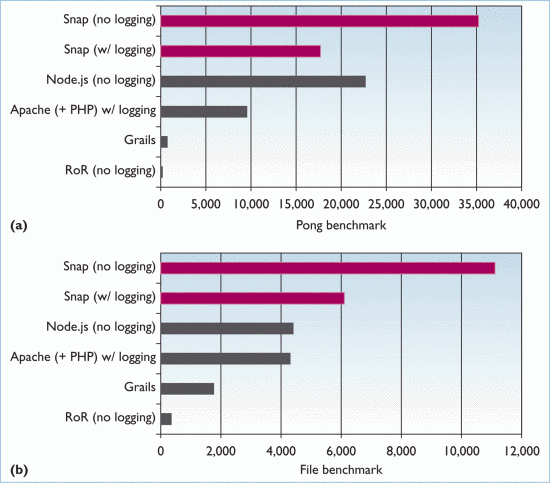
\includegraphics[width=0.7\textwidth]{final_report/pics/snapBenchmark.png}
    \caption{Snap and other frameworks, values are in requests per second \\ \textcopyright{} \citeyear{snapFramework} IEEE}
    \label{fig:snapBenchmark}
\end{figure}

Figure ~\ref{fig:snapBenchmark} shows the results of two benchmarks, one where a server
responded to a request by sending the string "pong", and another that records how fast
a server can send a 49 kilobyte image. As you can see in the
graph, for the file benchmark, the Snap framework was faster than all other frameworks.
Snap was only beaten by Node.js in the Pong benchmark when logging was turned on.
Turning logging off dramatically increased the performance of Snap, resulting in
Snap being 55\% faster than Node.js in the Pong benchmark. \parencite{snapFramework}

So, from the research done by \citeauthor{snapFramework}, we can see that Haskell
web frameworks can be significantly faster than more traditional web frameworks.
This is because Haskell uses the Glasgow Haskell Compiler (GHC). GHC compiles
Haskell programs into native machine code, ensuring high performance, especially
for concurrent programs such as web servers. Because of this, any Haskell web framework
that uses GHC, including Yesod, will serve requests faster than most traditional
web frameworks. \parencite{ghcSite}

\citeauthor{haskellWebComparison} published a blog post on his website with the
title \citetitle{haskellWebComparison}. In the post, \citeauthor{haskellWebComparison}
provides a quick comparison between some popular Haskell Web Frameworks, including
Yesod and Snap. The comparisons include the installation process of each framework,
the way they handle routing -- i.e. pointing a URL to a piece of code that will 
produce a response, and the quality of documentation for each framework. \parencite{haskellWebComparison}

At the end of his comparison, \citeauthor{haskellWebComparison} found that Yesod
was the best framework for his use case. One of the reasons for his choice was
because of the great documentation available for Yesod. The creator of Yesod
has written a book, \citetitle{haskellBook}, that is very comprehensive. The book
is available for free on the Yesod website. The amount of detail contained in this
book is also one of the reasons the Yesod web framework was chosen for this
project. \parencite{haskellWebComparison,yesodBook}

In \citetitle{beginnerYesod}, \citeauthor{beginnerYesod} discusses his experiences
in using Yesod as a beginner to the Haskell programming language. He mentions
the depth and thoroughness of the Yesod book when learning Yesod. However, when
making an actual website, he came across difficulties when trying to implement
features that required the use of functions not in the book. The author had
to check the documentation of the functions on Hackage, a Haskell package archive.
On Hackage, most functions contain a type signature and normally a one line
description. The author mentions how the type signatures would probably be
enough for experienced Haskell developers to work out how to use a function
but, as a beginner, founding out how a function works using types was much more
difficult. Because of this, the author had to spend a lot of time fixing type
errors. \parencite{beginnerYesod}

When first starting the project, I personally experienced the same issues described
in \citeauthor{beginnerYesod}'s blog post. I was not very good at reading the type
signatures available on Hackage, resulting in spending a lot of time fixing
unmatched type errors when trying to use functions not documented in the book.
However, as I became more experienced in Yesod and Haskell, these problems
became more and more rare as my understanding of Haskell type signatures increased.

\section{Real World Haskell Sites}

Some readers will be concerned about whether or not a Haskell web framework like
Yesod is ready for production websites. This is a valid concern considering the
relatively small amount of Haskell programmers when compared to mainstream 
programming languages. Readers will be pleased to know, however, that there
are some high traffic sites that are built using the Yesod web framework.

Freckle, previously known as Front Row Education, is an education
platform that provides a service to almost 10 million students \parencite{frontrowName}. 
In 2015, Freckle migrated their site to the Yesod web framework and have been 
using it ever since. \citeauthor{frontrow}, the CTO of Freckle, wrote an article
on his experience of using Yesod for a high traffic website. \parencite{frontrow}

In his article, \citeauthor{frontrow} states that the reason they chose a Haskell
Web Framework was because of the low resource usage and the ability to make
quick iterations that the Haskell language gives you. The article also discusses
how static typing saves time when writing unit tests. The developers at Freckle
did not have to deal with checking for null exceptions, mismatched types, and
other common bugs that are annoying to deal with. Spending less time dealing with
dynamic typing gives developers more time in implementing their features. The
modularity of Yesod also allows Freckle to reuse complex code, reducing potential
mistakes by developers, reducing the amount of code that needs to be written,
and allowing code to be updated quickly without the need to repeat changes. All
of these advantages allow developers to be more efficient and write fewer bugs. \parencite{frontrow}

However, there are some issues that the Freckle team came across during their migration.
Haskell builds are normally quite slow, as all external libraries used have to be
compiled during the build process. \citeauthor{frontrow} mentions that builds took
5-10 minutes on their most powerful machines. The author does mention that the team
could improve their build process by, for example, caching built files. The testing
suite caused problems for the team because when a test fails, they could not determine
which condition caused the failure when a test block has multiple conditions. The issue,
however, was reported to developers behind the testing library and the current
version of the testing suite does not have the issue mentioned in the article. The
lack of documentation for some functions also caused some frustration to the development
team, especially for the more junior developers who could not rely on type signatures. \parencite{frontrow}

When Freckle switched their main API to Yesod, their CPU usage rose to 95\%. This issue
did not occur during testing and profiling, in fact, the Freckle team were the first to
experience this particular issue. This is one issue when using a relatively niche language
like Haskell, you have to be comfortable with the idea that you may be the first person
to experience a particular issue. With other popular frameworks like Django, any issue
you discover has most likely been found and fixed by other members of the community.

Despite these issues, Freckle decided to stick with Yesod due to the advantages of the
Haskell compiler and the fact that the issues they experienced with regards to documentation
and build time are improving. And although the community is small, you can almost
always find help by asking on the StackOverflow or Google Groups pages or by visiting
the haskell-beginners IRC channel, an online chat room where developers new to haskell
can quickly and easily get help from some more experienced developers.
